Encontrar el área comprendida entre las curvas $y=x^2$ y $y=x^3$.

\nopagebreak
\begin{align*}
\text{Intersección: } x^2=x^3 \implies x^2(1-x)=0 \implies x=0, 1. \\
\text{En } [0,1], x^2 \ge x^3. \\
A &= \int_{0}^{1} (x^2 - x^3) \, dx \\
&= \left[ \frac{x^3}{3} - \frac{x^4}{4} \right]_{0}^{1} \\
&= \frac{1}{3} - \frac{1}{4} = \frac{1}{12}
\end{align*}

\[
\boxed{\displaystyle \frac{1}{12}}
\]

\begin{center}
    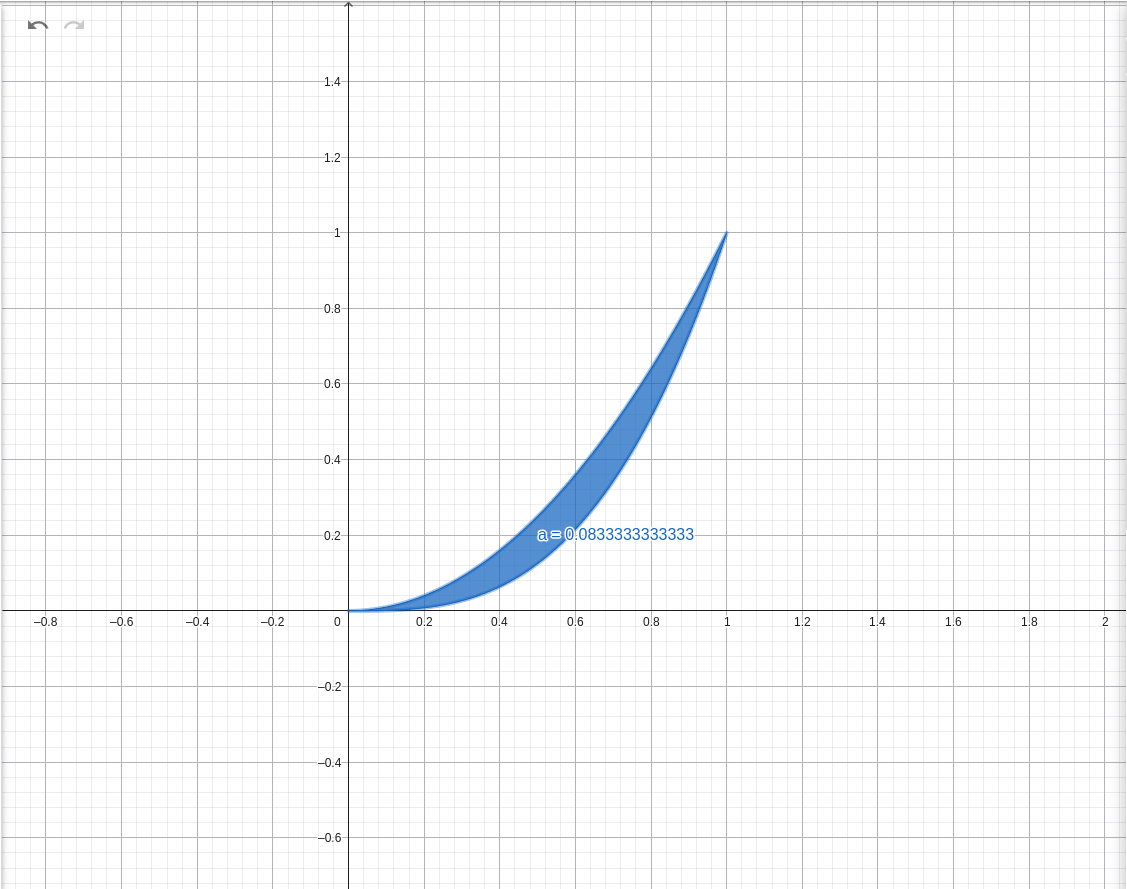
\includegraphics[width=0.5\textwidth]{Graficas/ejer25.png}
\end{center}
